\documentclass[useAMS, usenatbib, preprint, 12pt]{aastex}
\usepackage{cite, natbib}
\usepackage{float}
\usepackage{epsfig}
\usepackage{cases}
\usepackage[section]{placeins}
\usepackage{graphicx, subfigure}
\usepackage{color}
\usepackage{bm}

\newcommand{\columbia}{1}
\newcommand{\oxford}{2}
\newcommand{\uw}{3}
\newcommand{\princeton}{4}
\newcommand{\naigrain}{333}
\newcommand{\nmcquillan}{100}
\newcommand{\kepexample}{1430163}
\newcommand{\kepexampleperiod}{4}
\newcommand{\aigrainexampleperiod}{20.8}
\newcommand{\Kepler}{{\it Kepler}}
\newcommand{\kepler}{\Kepler}
\newcommand{\corot}{{\it CoRoT}}
\newcommand{\Ktwo}{{\it K2}}
\newcommand{\ktwo}{\Ktwo}
\newcommand{\TESS}{{\it TESS}}
\newcommand{\LSST}{{\it LSST}}
\newcommand{\SDSS}{{\it SDSS}}
\newcommand{\PLATO}{{\it PLATO}}
\newcommand{\Teff}{$T_{\mathrm{eff}}$}
\newcommand{\teff}{$T_{\mathrm{eff}}$}
\newcommand{\FeH}{[Fe/H]}
\newcommand{\feh}{[Fe/H]}
\newcommand{\ie}{{\it i.e.}}
\newcommand{\eg}{{\it e.g.}}
\newcommand{\logg}{log \emph{g}}
\newcommand{\dnu}{$\Delta \nu$}
\newcommand{\numax}{$\nu_{\mathrm{max}}$}
\newcommand{\acfRMS}{1.45}
\newcommand{\pgramRMS}{1.10}
\newcommand{\mcmcRMS}{0.87}

\begin{document}

\title{Inferring stellar rotation periods using Gaussian processes}

\author{%
   Ruth Angus\altaffilmark{\columbia},
   Suzanne Aigrain\altaffilmark{\oxford},
   Timothy Morton\altaffilmark{\princeton}
   \& Daniel Foreman-Mackey\altaffilmark{\uw}
}

\altaffiltext{\columbia}{Simons Fellow, Department of Astronomy, Columbia
University, NY, NY, RuthAngus@gmail.com}
\altaffiltext{\oxford}{Subdepartment of Astrophysics, University of Oxford,
UK}
\altaffiltext{\uw}{Department of Astronomy, University of Washington, Seattle,
WA}
\altaffiltext{\princeton}{Department of Astrophysical Sciences, Princeton University,
Princeton, NJ}

\begin{abstract}
The light curves of spotted, rotating stars are often non-sinusoidal and
quasi-periodic---spots are not static on the stellar surface and have finite
lifetimes causing stellar flux variations to slowly shift in phase.
A strictly periodic sinusoid is therefore not a representative model for the
light curve of star with a rotational signal.
Ideally, a physical model of the stellar surface would be conditioned on the
data, however the parameters of such models can be highly degenerate
\citep[\eg][]{Russell1906, Jeffers2009}.
Instead, we use an appropriate {\it effective} model: a Gaussian Process (GP)
with a quasi-periodic covariance kernel function.
By modelling the light curve with a GP, a highly flexible semi-parametric
function, we avoid the necessity of choosing a `best fitting' functional form,
whilst sampling directly from the posterior Probability Density Function (PDF)
of the periodic parameter and marginalising over the other kernel
hyperparameters.
We used \naigrain\ simulated light curves with a range of rotation periods
to test the GP model.
We attempted to recover the rotation periods using three methods: our GP
method, a sine-fitting periodogram method and an AutoCorrelation Function
(ACF) method.
The posterior PDF of the rotation period parameter was sampled using the
affine invariant ensemble Markov Chain Monte Carlo (MCMC) sampler {\tt emcee}
\citep{Foreman-Mackey2013}, and the GP operations were performed using the
{\tt george} python package \citep{George}.
Rotation periods inferred via this method are more precise and accurate than
the periodogram and ACF methods.
Furthermore, rotation periods are inferred probabilistically, allowing them to
be easily incorporated into follow-on studies; inferring stellar ages or
characterising star-planet interactions for example.
In addition, unlike the sine-fitting periodogram and ACF methods, the
posterior PDF samples allow for proper characterisation of uncertainties.
This method eliminates the need to define a heuristic detection criterion such
as are often used in the literature: a light curve that does not contain a
rotation signal will return the prior PDF.

% Furthermore, the improvement is expected to be even more dramatic when applied
% to real, noisy {\it Kepler} light curves, since the GP method is well suited
% to modelling rotation signals and correlated noise simultaneously.

\end{abstract}

\section{Introduction}

The light curves of spotted, rotating stars are often non-sinusoidal and
Quasi-Periodic (QP).
These stars vary in brightness due to active regions on their surfaces which
rotate in and out of view.
The non-sinusoidal quality is caused by the complicated surface spot patterns
and the quasi-periodicity is produced both by the finite lifetimes of these
active regions and the presence of differential rotation on the stellar
surface.
A strictly periodic sinusoid is therefore not a good model for stellar light
curves.
In an ideal world, a physical model of the stellar surface would be
conditioned on the data.
A physically realistic model would perfectly capture the complexity of shapes
within stellar light curves as well as the quasi-periodic nature, allowing for
extremely precise probabilistic period recovery.
However, such physical models require many free parameters in order to
accurately represent a stellar surface and some of these parameters are
extremely degenerate \citep[\eg][]{Russell1906, Jeffers2009}.
In addition to global stellar parameters such as inclination and rotation
period, each spot or active region should have (at minimum) a longitude,
latitude, size, temperature and lifetime.
Considering that many stars have on the order of hundreds of spots, the number
of free parameters quickly becomes unwieldy, especially if the posterior PDFs
of these parameters are explored with MCMC.
Simplified spot models, such as the one described in \citet{Lanza2014} where
only two spots are modelled, have produced successful results, however these
simplified models sacrifice some precision due to lack of model flexibility.
Instead of using a physical model for stellar light curves, we choose to use
an {\it effective} model: one which captures the behaviour but is not
physically motivated, although the parameters of this model may be {\it
interpreted} as physical ones.
An ideal effective model for the light curve of a spotted, rotating star is
one with a small number of non-degenerate parameters that is flexible enough
to perfectly capture non-sinusoidal, QP behaviour.
These requirements are fulfilled by a Gaussian process (GP) model.

The standard methods used for measuring rotation periods include detecting
peaks in a Lomb-Scargle \citep{Lomb1976, Scargle1982} (LS) periodogram
\citep[e.g.][]{Reinhold2013}, Auto-Correlation Functions (ACFs)
\citep{Mcquillan2013} and wavelet transforms \citep{Garcia2014}.
The precision of the LS periodogram and wavelet methods are limited by the
suitability of the model choice.
A sinusoid is used in the case of the LS periodogram and the wavelet method
relies on a choice of mother wavelet that is assumed to describe the data over
a range of transpositions \citep[see, \eg][]{Carter2010}.
In contrast, the ACF method is much better suited to signals that are
non-sinusoidal.
In fact, it doesn't matter what shape the signal is: as long as it is
approximately periodic the ACF will display peaks located at the rotation
period.
A drawback of the ACF method however, is that it requires data to be
evenly-spaced\footnote{\citet{Edelson1988} describe a method for computing
ACFs for unevenly-spaced data.} which is not the case with \Kepler\ light
curves (although in many cases it can be approximated as uniformly sampled).
An ACF is also an operation performed on the data, not a generative model of
the data and is therefore not inherently probabilistic.
For this reason it is very difficult to estimate the uncertainty on an ACF
rotation period measurement.
% Many rotation periods in the literature have been inferred by measuring the
% position of the first peak in an ACF, however this approach can be dangerous.
% The exponential decay in correlation can shift the peak position short-wards
% of its true value, leading to an underestimate of the period.
% We return to this point in section \textsection \ref{sec:discussion}.

The motivation for developing a GP-based method for rotation period inference
is, firstly to measure more accurate and precise rotation periods using a
better-suited generative model than a sinusoid for the reasons explained
above.
Secondly, in order to infer {\it probabilistic} periods, i.e. to estimate the
posterior PDF of the rotation period and thereby produce a realistic and
estimate of its uncertainty.
Thirdly, to allow for an additional correlated noise model to be included
during regression, the parameters of which could be marginalised over.
% And fourthly to provide some way of determining whether a periodic model is
% supported by the data over a purely stochastic one.

GPs are commonly used in the machine learning community and increasingly
in other scientific fields, for example biology and geophysics.
More recently, GPs have been used in the astronomy literature \citep[see
\eg][]{Gibson2012, Haywood2014, Haywood2015, Evans2015, Rajpaul2015,
Rajpaul2016, Aigrain2016}.
% FIXME: CITATIONS Gibson, Aigrain, Evans, Rajpaul, Waldman(?), Cosmology,
% geology, biology, Rasmussen & Williams, etc.
They are useful in regression problems involving any stochastic process,
specifically when the probability distribution for the process is a
multi-variate Gaussian.
If the probability of obtaining a data-set is a Gaussian in $N$ dimensions,
where $N$ is the number of data points, that data-set can be described as, and
with, a Gaussian process.
An in-depth introduction to Gaussian processes is provided by
\citet{Rasmussen2005}.

GP models parameterise the covariance between data points and a kernel
function provides the form of covariance matrix parameterisation.
For example, take the time-series in figure \ref{fig:GP_example}.
This is the \kepler\ light curve of KIC \kepexample, a relatively active star that
rotates once every $\sim$ 4 days.
The stochastic variability in this time-series is typical of \kepler\ FGK
stars.
Clearly, data points in this light curve are correlated.
Points that are close together in time are tightly correlated and those that
are widely separated in time are loosely correlated.
The way in which the covariance varies with the separation between data points
is modelled when using GP regression; it is not the data but the {\it
covariance structure} that is modelled.
This fact is what gives GPs their flexibility---they can model any time
series with a similar covariance structure.
In addition, a very simple function can usually capture the covariance
structure of a light curve, whereas a much more complicated one may be
required to model the time-series itself.
% The light curve of \Kepler-452 has been modelled with a GP in figure
% \ref{fig:GP_example}, shown in orange.
In figure \ref{fig:GP_example} the light curve of KIC \kepexample\ has been
modelled with a GP.
% Both provide adequate fits to the data, however only the periodic kernel
% function, `QP' is a useful model because it has a periodic parameter.
% I return to this point shortly.

A range of kernel functions could be used to describe stellar variability.
For example, the simplest and most commonly used kernel function, the `Squared
Exponential' (SE) produces an adequate fit to the KIC \kepexample\ light
curve.
The SE kernel function is defined as,
\begin{equation}
k_{i,j} = A \exp \left(-\frac{(x_i - x_j)^2}{2l^2} \right).
\end{equation}
\label{eq:SE}
Here $A$ is the amplitude of covariance, $l$ is the length scale of
exponential decay and $x_i-x_j$ is the separation between data points.
The SE kernel function has the advantage of being very simple---it has just
two parameters, a covariance amplitude and length scale: $A$ and $l$.
If $l$ is large two data points far apart in $x$ will be tightly correlated,
and if small they will be loosely correlated.
Another property of the SE kernel function is that it produces functions that
are infinitely differentiable.
It is therefore possible to model a data set and its derivatives
simultaneously.
% \citep[see \eg][]{Rajpaul2015}
The SE kernel function is not a good model of the covariance in stellar light
curves, nor a {\it useful} one for the problem of rotation period inference
because it does not capture periodic behaviour.
In order to infer rotation periods it is necessary to use a periodic kernel
function.
For this reason, we use the `Quasi-Periodic' kernel function.
The QP kernel function is defined as
\begin{equation}
k_{i,j} = A \exp \left(-\frac{(x_i - x_j)^2}{2l^2} -
\Gamma^2 \sin^2(\frac{2\pi}{P}) \right).
\end{equation}
\label{eq:QP}
It is the product of the SE kernel function, which describes the overall
covariance decay, and an exponentiated, squared, sinusoidal kernel function
that describes the periodic covariance structure.
$P$ can be interpreted as the rotation period of the star and $\Gamma$
controls the amplitude of the $\sin^2$ term.
If $\Gamma$ is very small, only points almost exactly one period away are
tightly correlated and points that are slightly more or less than one period
away are very loosely correlated.
If $\Gamma$ is large, points separated by one period are tightly
correlated and points separated by slightly more or less are still highly
correlated although less so.
This kernel function allows two data points that are separated in time by one
rotation period to be tightly correlated, while points separated by half a
period can be weakly correlated.
We also use an extra parameter, $\sigma$ which is an additional white noise
term added to the diagonal elements of the covariance matrix.
It is the fraction by which the observational uncertainties have been
underestimated --- if the uncertainties reported on the data are too small,
this parameter will be non-zero.
In practice however, this parameter should always be non-zero when performing
GP regression.
This is because the covariance matrix must be positive definite, however
matrix inversion performed using most solvers is approximate, not exact,
therefore slight deviations from positive definiteness can arise.
Including a small amount of extra variance in the model allows enough
flexibility that the matrix inversion algorithms do not run into numerical
issues.

This QP kernel function was used to produce the model shown in figure
~\ref{fig:GP_example}.

In order to infer a stellar rotation period from a light curve, we fit a GP
model with a QP kernel function to the data.
The likelihood of the model, conditioned on the data could then be maximised
in order to find the maximum likelihood value for $P$.
In this study however, the full posterior PDFs of the parameters are explored
using MCMC.
This approach comes at a cost: a GP model is expensive to compute once as it
requires an inversion and determinant evaluation of the covariance matrix, let
alone the many thousands of times that is necessary to fully explore the
posteriors of the parameters.
Fully exploring the posterior PDF of $P$ is important however, as it provides
an accurate estimate of the uncertainty on the rotation period.

\begin{figure}
\begin{center}
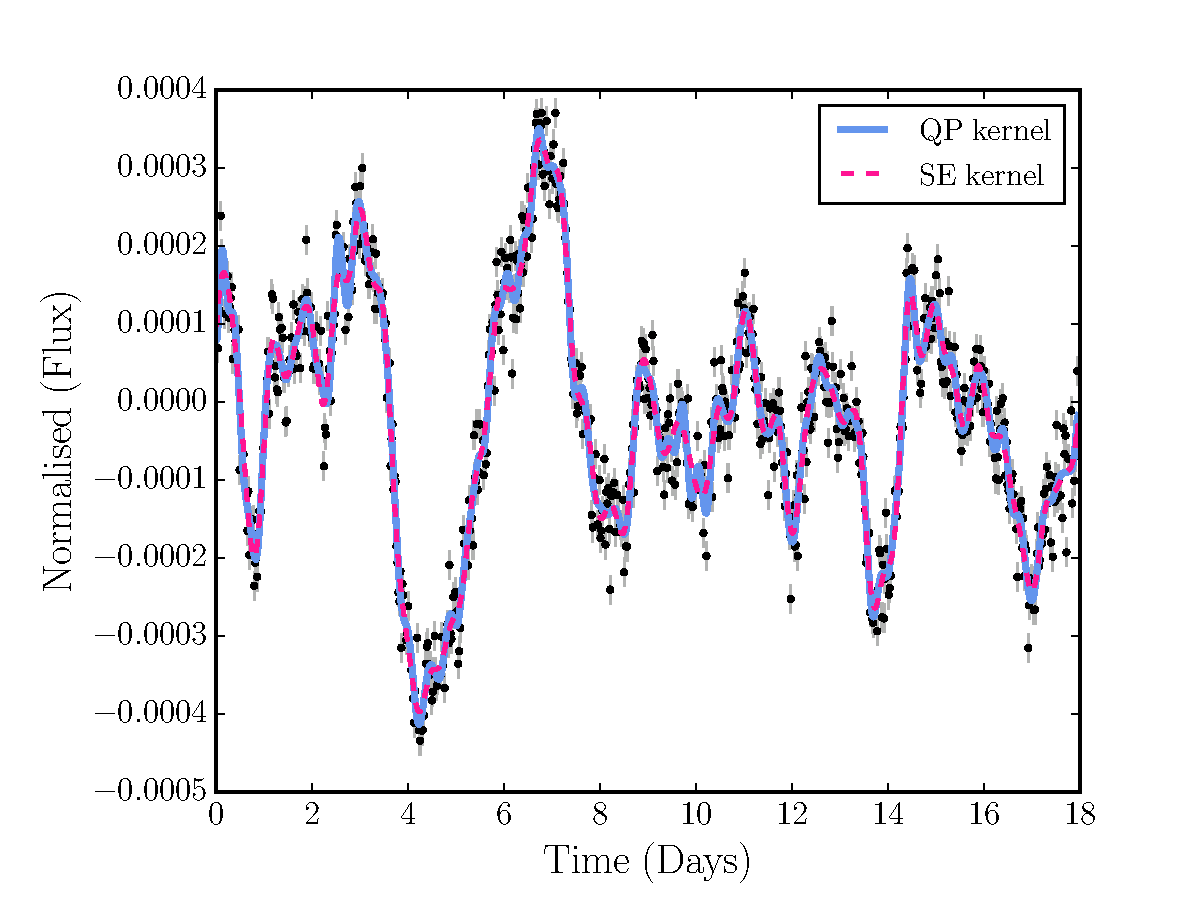
\includegraphics[width=6in, clip=true]{figures/001430163.pdf}
\caption[A light curve with a GP model.]
{Light curve of KIC \kepexample, an active star with a rotation period of
$\sim$ \kepexampleperiod\ days.
The blue line shows a fit to the data using a Gaussian process model with a QP
covariance kernel function.}
\label{fig:GP_example}
\end{center}
\end{figure}

In \textsection \ref{sec:simulations} of this paper we describe the simulated
light curves used to test rotation period inference methods.
In \textsection \ref{sec:method} we describe the various methods used to
recover the rotation periods: the periodogram, ACF and GP methods.
In \textsection \ref{sec:kepler} we apply our method to real \kepler\ data and
the results of the paper are discussed in \textsection \ref{sec:discussion}.

\section{Simulated light curves}
\label{sec:simulations}

In order to test the GP method we attempted to the measure rotation periods of
a set of simulated light curves.
We used \naigrain\ light curves generated for the \citet{Aigrain2015}
`hare and hounds' rotation period recovery experiment.
These light curves were simulated by placing dark, circular spots with slowly
evolving size, on the surface of bright, rotating spheres, ignoring
limb-darkening effects.
\citet{Aigrain2015} simulated one thousand light curves in order to test the
ability of participating teams to recover both the stellar rotation periods
and the rotational shear: the amplitude of surface differential rotation.
% Since we are not interested in recovering differential rotation we only used
% those light curves simulated {\it without} differential rotation, of which
% there are \naigraincurves.
For the purpose of demonstrating that our method can recover rotation periods,
we selected only the \naigrain\ out of the 1000 without differential
rotation.
We opted to use only solid-body rotators because differential rotation may
produce some additional scatter in the rotation period measurements recovered.
In future we intend to test whether we can recover differential rotation using
the GP method and will then use the full set of 1000 light curves.
The distributions of input parameters used to generate these light curves are
listed in \citet{Aigrain2015}.
Light curves were simulated with a real \Kepler\ long-cadence time array:
one data point every thirty minutes over a four year duration.
90\% of the rotation periods of the simulations were randomly drawn from a
log-uniform distribution between 10 and 50 days and 10\% from a log-uniform
distribution between 1 and 10 days.
A histogram of the \naigrain\ solid-body rotation periods is shown in figure
\ref{fig:period_hist}.
The light curves were also generated with a range of stellar inclination
angles, activity levels, spot lifetimes and more.
Once simulated, the light curves were added to real \kepler\ light curves with
no obvious astrophysical variability in order to preserve the noise properties
of the time series.
Figure \ref{fig:demo_lc} shows an example of a simulated light curve with a
period of \aigrainexampleperiod days.

The ranges and distributions of the physical stellar parameters used in the
simulated light curves are tabulated below, in table
\ref{tab:simulation_parameters}, and figure \ref{fig:period_hist} shows the
distribution of rotation periods in the \citet{Aigrain2015} sample.

\begin{table*}
\begin{center}
\caption{Ranges and distributions of parameters used to simulate light curves
in \citet{Aigrain2015}}
\begin{tabular}{lcc}
\hline\hline
    Parameter & Range & Distribution \\
    \hline
    Rotation period, $P_{rot}$ & 10 - 50 days (90\%) & log uniform \\
    & 1 - 10 days (10\%) & log uniform \\
    Activity cycle length & 1 - 10 years & log uniform \\
    Inclination & 0 - 90$^\circ$ & Uniform in $\sin^2i$ \\
    Decay timescale & (1 - 10) $\times P_{rot}$ & log uniform \\
\hline
\end{tabular}
\end{center}
\end{table*}
\label{tab:simulation_parameters}

\begin{figure}
\begin{center}
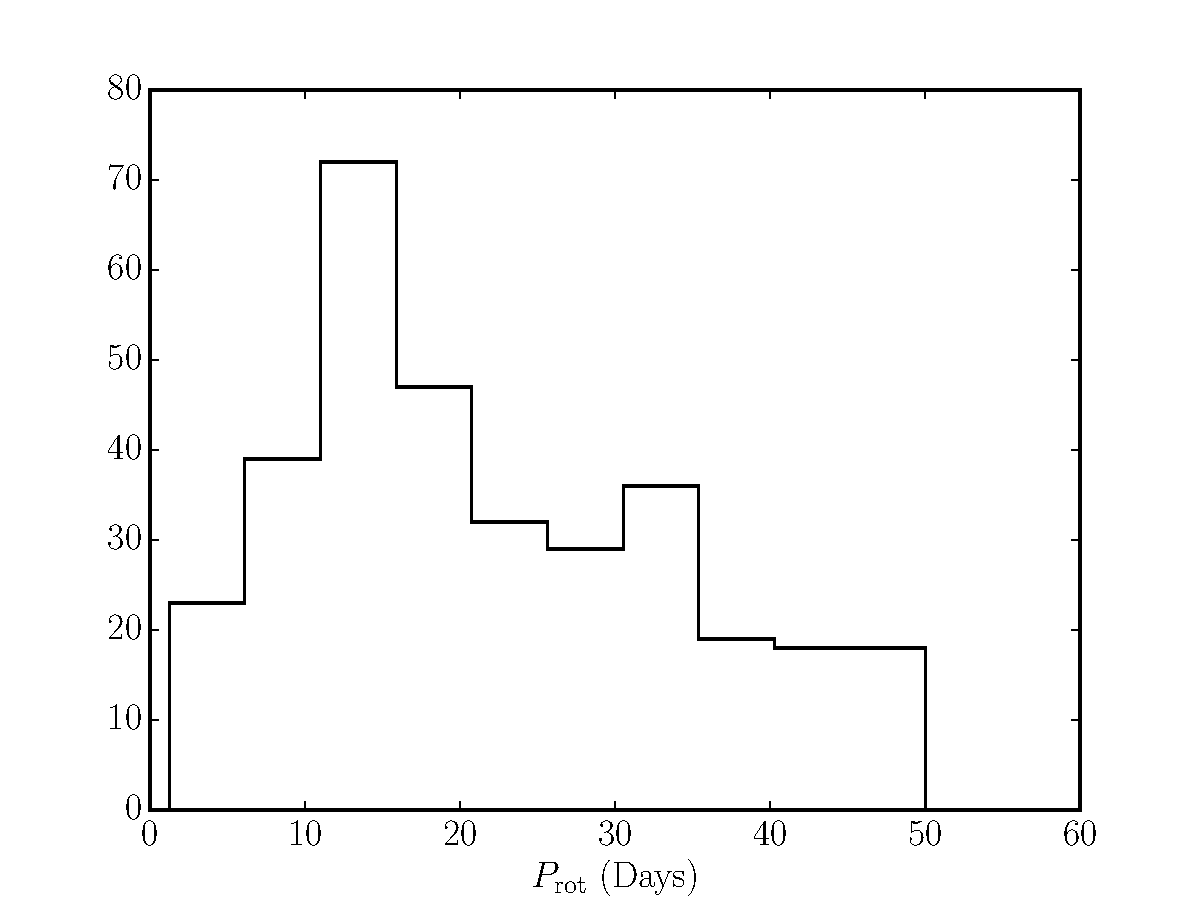
\includegraphics[width=6in, clip=true]{figures/period_hist.pdf}
\caption{A histogram of the rotation periods used to generate the \naigrain\
simulated light curves in \citet{Aigrain2015}.}
\label{fig:period_hist}
\end{center}
\end{figure}

\begin{figure}
\begin{center}
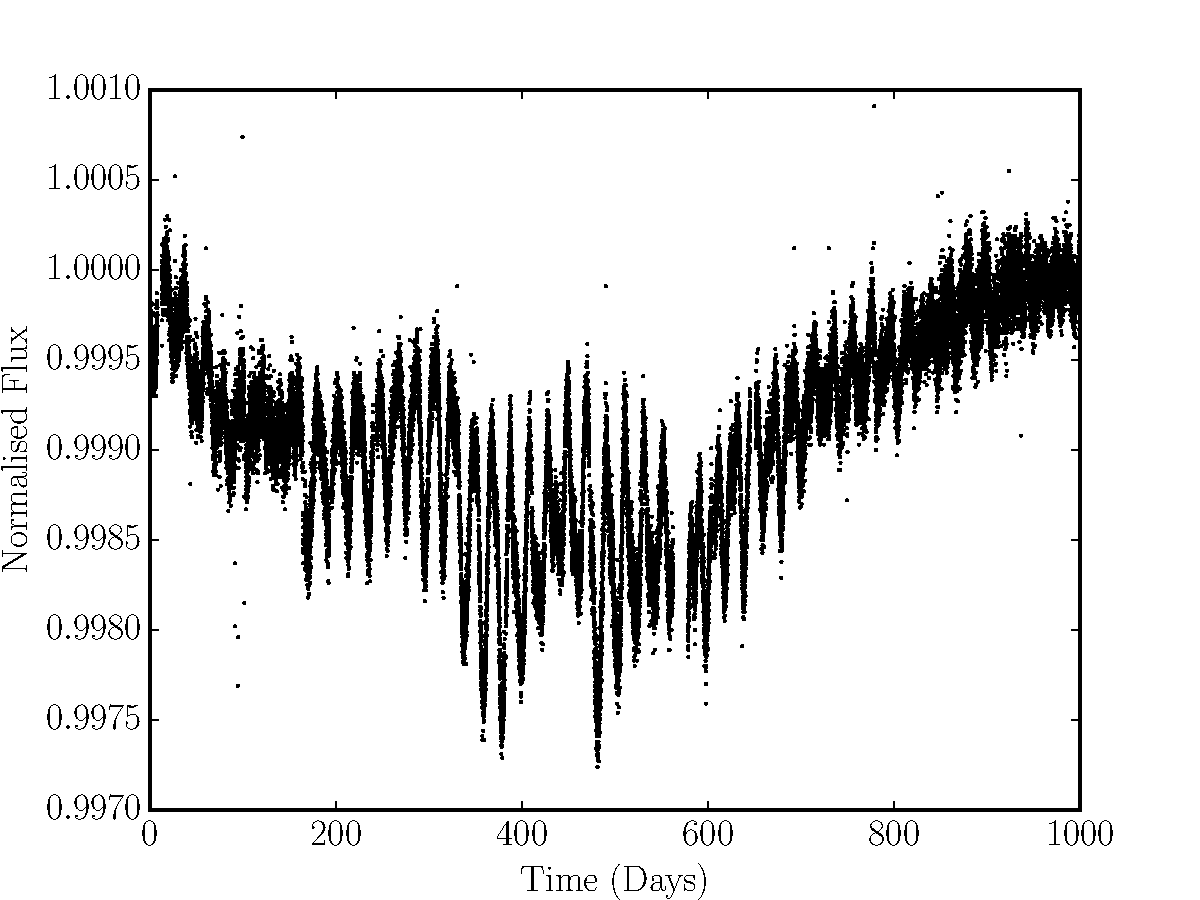
\includegraphics[width=6in, clip=true]{figures/demo_lc.pdf}
\caption[A simulated light curve.]
{An example simulated light curve. This `star' has a rotation period of
\aigrainexampleperiod\ days.}
\label{fig:demo_lc}
\end{center}
\end{figure}

% We attempted to recover the rotation periods of these \naigrain\ light curves
% using three methods: the ACF method; the LS periodogram method; and the GP
% method, and compared their performances.

\section{Rotation period recovery}
\label{sec:method}
\subsection{ACF}

We calculated an ACF for each light curve following the method of
\citet{Mcquillan2013}.
An ACF is calculated for each light curve and smoothed by convolving with a
Gaussian with $\sigma=9$ days.
A rotation period is estimated as the lag-time of the highest peak in the ACF,
less than 100 days.
This is not always the first peak: the second can be larger than the first if
there are two active regions at or near opposite longitudes on the surface of
the star---producing a light curve with two dips per rotation period.
We restrict our search to periods less than 100 days because this is the
maximum period that is realistically recoverable in \kepler\ light curves ---
instrumental noise significantly distorts signals on longer timescales.
An example ACF of the light curve in figure~\ref{fig:demo_lc} is shown
in figure \ref{fig:demo_acf}.

\begin{figure}
\begin{center}
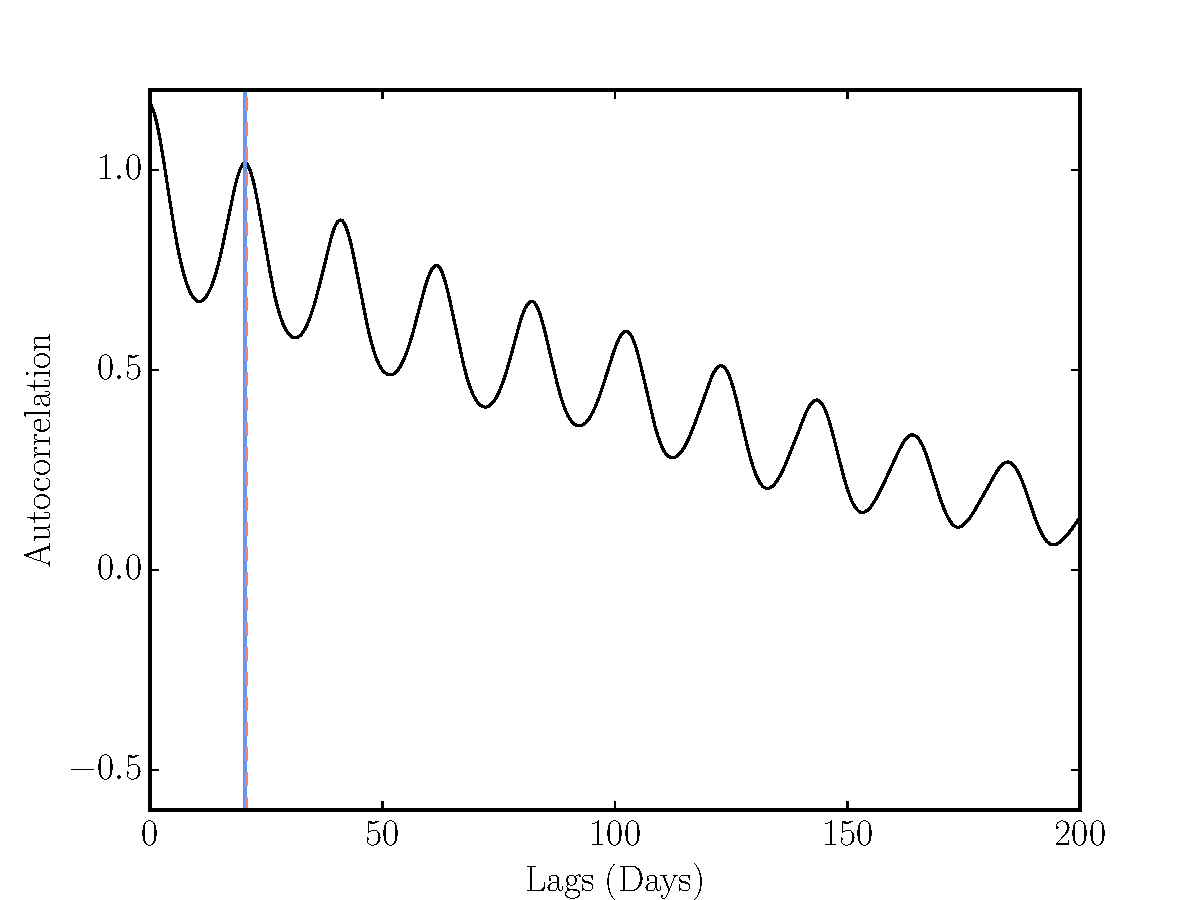
\includegraphics[width=6in, clip=true]{figures/demo_ACF.pdf}
\caption[ACF of a simulated light curve.]
{An autocorrelation function of the simulated light curve shown in figure
\ref{fig:demo_lc}.
The vertical blue line shows the period measured using the ACF method (20.4
days) and the pink dashed line shows the period that was used to simulate the
light curve (\aigrainexampleperiod\ days).}
\label{fig:demo_acf}
\end{center}
\end{figure}

The ACF method has proven to be extremely useful for measuring rotation
periods.
The catalogue of rotation periods of \Kepler\ stars provided in
\citet{Mcquillan2013} has been widely used by the community and has provided
ground-breaking results for stellar and exoplanetary science.
The results of the ACF method as tested in \citet{Aigrain2015} were positive
(see, for example their figure 8) as it produced a large number of accurate
rotation period measurements.
Another advantage of the ACF method is that it is fast to implement.
A clear disadvantage however, as already mentioned above, are the poorly
defined uncertainties for rotation periods estimated using an autocorrelation
function.
This is related to the fact that ACF period detection is a non-probabilistic
method, another drawback of ACF periods.

We applied the ACF method to the sample of \naigrain\ simulated light
curves.
Periods measured using the ACF method are plotted against the original
rotation period values used to generate the light curves in figure
\ref{fig:compare_acf}.
The $2n$ and $\frac{1}{2}n$ harmonic lines are shown as dashed lines.
The RMS scatter about the $x=y$ line for rotation periods measured using the
ACF method is \acfRMS.
The agreement between the injected and recovered rotation periods is good in
general, however twice the true rotation period is often found.
In addition, some rotation periods are drastically over- and underestimated.
Of the points clustered close to the $x=y$ line, more fall slightly below it
than above it, \ie\ rotation periods are preferentially underestimated.
This is a feature of the peak position measurement method that is performed on
the ACF.
ACFs of stellar light curves are similar to the QP kernel function in equation
\ref{eq:QP}: periodic functions added to decaying exponentials.
In such functions the peak positions can be shifted towards the left, the
short period end, because the decaying exponential raises the left side of
each peak more than the right.
It is possible to model this effect, however the standard practice is to
simply measure the peak position without taking it into account.
We adopt the standard practice approach here in order to provide a comparison
between our new method and that used largely in the literature.

\begin{figure*}
\begin{center}
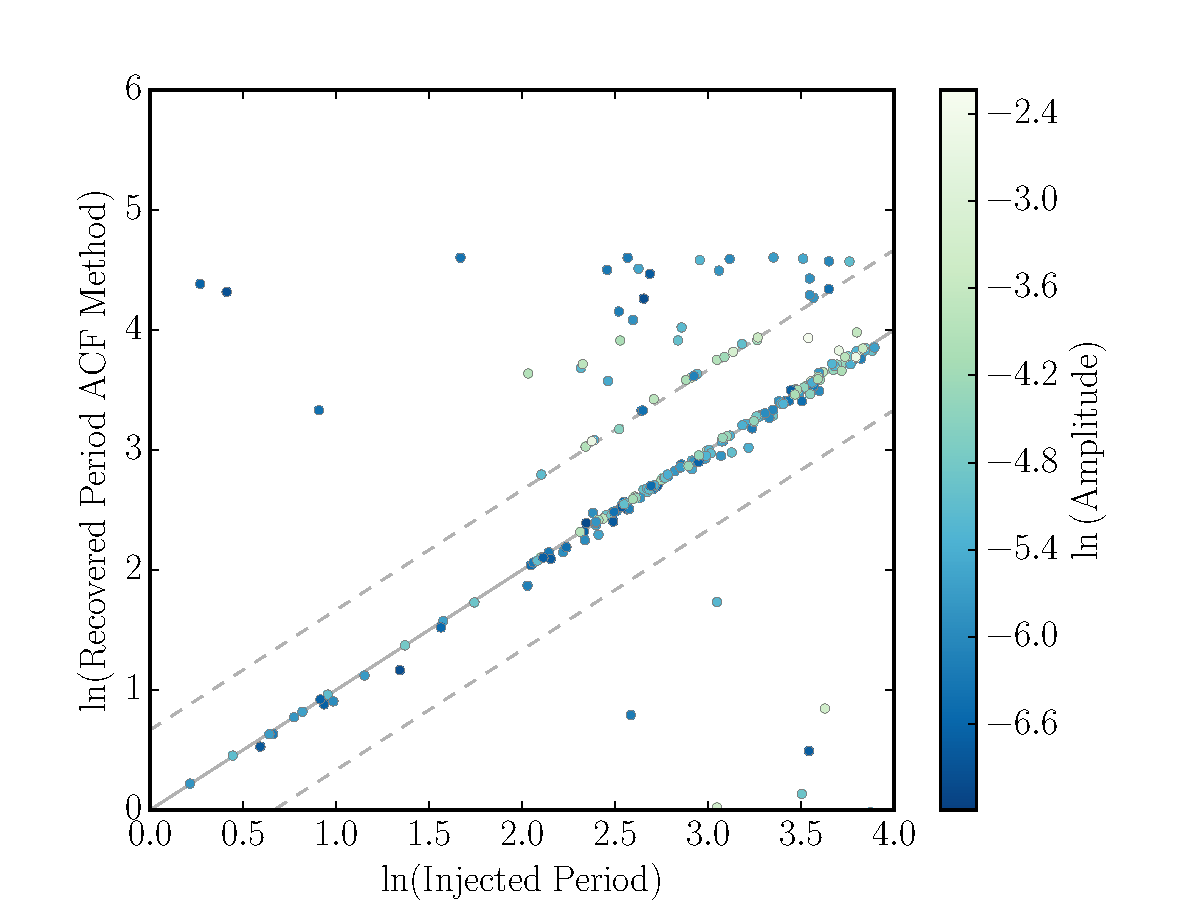
\includegraphics[width=6in, clip=true]{figures/compare_acf.pdf}
\caption[ACF results.]
{The `true' rotation periods used to generate \naigrain\ simulated light
curves vs the rotation periods measured using the ACF technique.}
\label{fig:compare_acf}
\end{center}
\end{figure*}

\subsection{LS periodogram}

For each simulated light curve, a LS periodogram
\footnote{LS periodograms were calculated using the gatspy Python module:
\url{https://github.com/astroML/gatspy/tree/master/gatspy/periodic}.}
was computed over a grid of 10,000 periods, evenly spaced in frequency,
between 1 and 100 days.
The period of the highest peak in the periodogram was adopted as the rotation
period.
The resulting recovered rotation periods are plotted as a function of the true
periods in figure \ref{fig:pgram_compare}.
The RMS scatter for rotation periods measured using the LS periodogram
technique is \pgramRMS.
The longer-period measurements provide the dominant contribution to this RMS.
% We believe that the unsuccessful recoveries occurring preferentially for
% shorter rotation periods are produced by additional, longer timescale
% variations in some of the light curves.
% Specifically, by fluctuations produced by changes in the total spot coverage
% on the stellar surface.
% These fluctuations can occasionally be larger in magnitude than those produced
% by the rotational signal itself and are present in the majority of outlying
% light curves that occupy the top left of figure
% \ref{fig:pgram_compare_noise-free}.

\begin{figure*}
\begin{center}
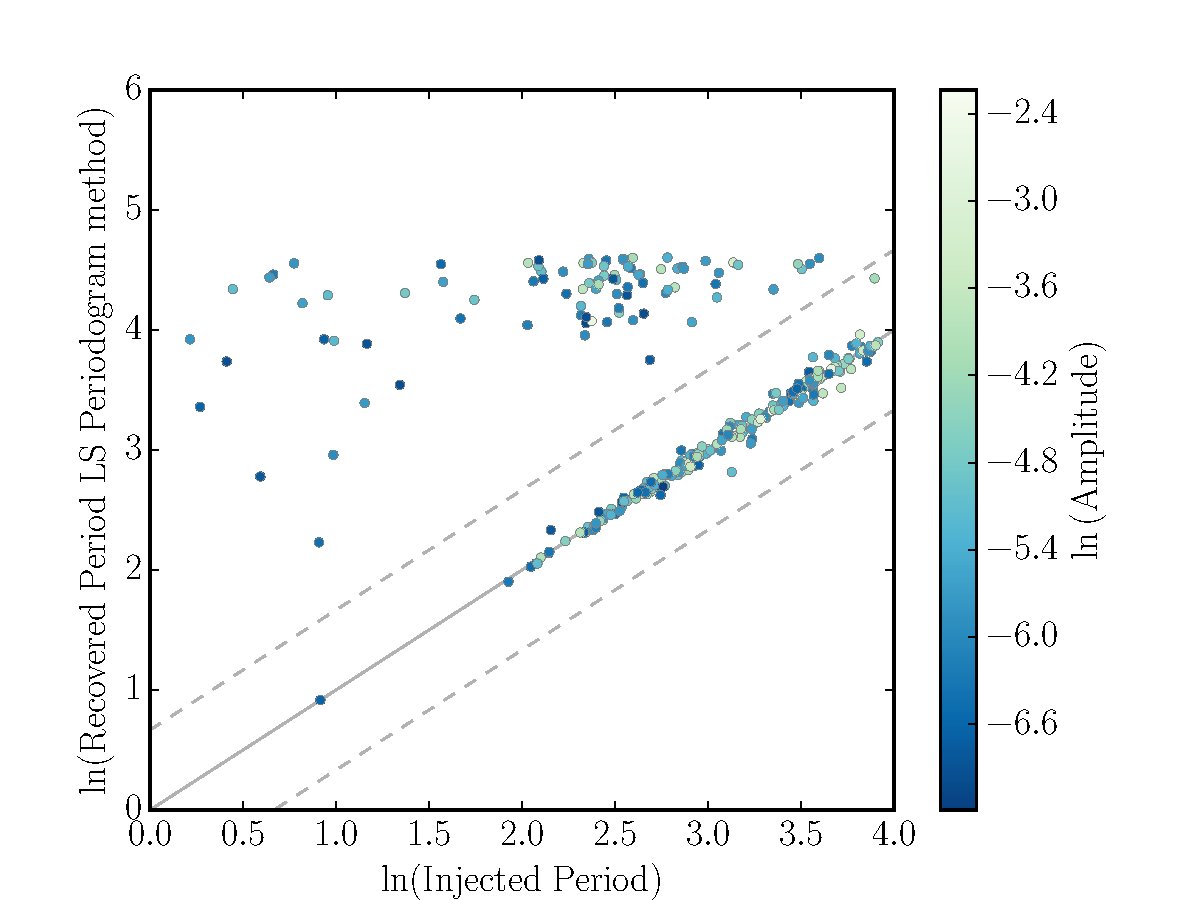
\includegraphics[width=6in, clip=true]{figures/compare_pgram.pdf}
\caption[LS periodogram results.]
{The `true' rotation periods used to generate \naigrain\ simulated light
curves vs the rotation periods measured using a LS periodogram technique.}
\label{fig:pgram_compare}
\end{center}
\end{figure*}

\subsection{The GP method}

In order to recover the rotation period of a simulated light curve using
Gaussian processes, we sample the following posterior PDF:
\begin{equation}
p({\bm \theta}\,|\,y) \propto \mathcal L(y\,|\,{\bm \theta}) p({\bm \theta}),
\end{equation}
\label{eq:posterior}
where $y$ are the light curve data, $\bm \theta$ are the hyperparameters 
of the kernel described in equation \ref{eq:QP}, $\mathcal L$ is the 
GP likelihood function, and $p({\bm \theta})$ is the prior on the 
hyperparameters.  The GP likelihood is similar to the simple Gaussian likelihood
function used for optimisation problems where the uncertainties are
Gaussian and uncorrelated. The latter can be written
\begin{equation}
\ln \mathcal{L} = -\frac{1}{2}\sum_{n=1}^N\frac{(y_n-\mu)^2}{\sigma_n^2}
    - \frac{N}{2}\ln(2\pi\sigma_n^2),
\end{equation}
\label{eq:chi2}
where $y_n$ are the data, $\mu$ is the mean model and $\sigma_n$ are the
Gaussian uncertainites on the data.
The equivalent equation in matrix notation is
\begin{equation}
\ln \mathcal{L} = -\frac{1}{2}\bf{r}^T\bf{C}^{-1}\bf{r}-\ln|\bf{C}|
    + \mathrm{constant},
\end{equation}
\label{eq:lhf1}
where $\bf{r}$ is the vector of residuals and $\bf{C}$ is the covariance
matrix,
\begin{eqnarray}
	\mathbf{C} &=& \left (\begin{array}{cccc}
	\sigma^2_1 & \sigma_{2, 1} & \cdots & \sigma_{N, 1} \\
	\sigma_{1, 2} & \sigma^2_2 & \cdots & \sigma_{N, 2} \\
    && \vdots & \\
	\sigma_{1, N} & \sigma_{2, N} & \cdots & \sigma^2_N
\end{array}\right )
\end{eqnarray}
In the case where the uncertainties are uncorrelated, the noise is `white',
(which is a frequent assumption made by astronomers and is sometimes
justified) and the off-diagonal elements of the covariance matrix are zero.
However, in the case where there is evidence for correlated
`noise'\footnote{In our case the `noise' is actually the model!}, as in the
case of \Kepler\ light curves, those off-diagonal elements are non-zero.
With GP regression, a covariance matrix generated by the kernel function,
${\bf K}$ replaces ${\bf C}$ in the above equation.
Incidentally, this approach is the reverse of the regression techniques
usually employed by astronomers.
In most problems in astronomy one tries to infer the parameters that describe
the mean model and, if correlated noise is present, to marginalise over that
noise.
Here, the parameters describing the correlated noise are what we are
interested in and our mean model is simply a straight line at $y=0$.

Sampling the posterior described above presents several challenges:
\begin{itemize}
\item Evaluating $\mathcal L$ for an entire \Kepler\ lightcurve 
($\sim$40,000 points) takes about $\sim$5\,s--- too computationally expensive 
to perform inference on large numbers of light curves\footnote{All computational
times cited in this section are based on evaluations on a 
single core of a 2015 Macbook Pro, 3.1 GHz Intel Core i7.}.  The matrix operations
necessary to evaluate the GP likelihood (using the fast matrix solver 
HODLR \citep{Ambikasaran2014}, implemented in the {\tt george} \citep{George} 
python package) scale as $N\ln(N)^2$, where $N$ is
the number of data points in the light curve.

\item The flexibility of this GP model allows for insidious kinds of 
posterior multimodality and "over-fitting"--like behavior.  For example, 
if $l$ is small,  the non-periodic factor in the covariance kernel may dominate, 
allowing for a good fit to the data without requiring any 
periodic covariance structure---even if
clear periodic structure is present.  Additionally, if $\Gamma$ is too large,
then [explain in more technical terms that "the GP gets way too wiggly and
overfits the data without caring about the periodicity." ]

\item In some cases, the posterior may also be multi-modal in period---that is, 
there may be significant posterior density at half or twice the true period $P$.
This is related to how the ACF method must guard against identifying periods 
at half or twice the true period. 
\end{itemize}

We address the first of these difficulties in two distinct ways: subsampling
the data and splitting the light curve into independent sections.  
To subsample, we randomly select 1/30th of the points in the full light curve (an 
average of $\sim$1.5 points per day).  This decreases the likelihood evaluation 
time by a factor of about 50, down to about 100\,ms.
We then split the light curve into equal-sized
chunks containing approximately 300 points per section (corresponding to about
200 days), and evaluate the log-likelihood as the sum of the log-likelihoods
of the individual sections (all using the same parameters $\theta$).  This reduces
computation time because the section-based likelihood evaluation scales as $mn\ln(n)^2$, where $n$ is the number of data points per section and $m$ is the number of sections.
This method further reduces computation time for a typical light curve (subsampled
by a factor of 30) by about a factor of two, to about 50\,ms.

In order to manage the extreme flexibilty of the GP model and focus on 
reliably retrieving the period parameter, we also impose priors
on the non-period GP parameters that we 
learned during the development of this method.  
Beginning with very broad priors (uniform in log space between 
-20 and 20) on all the parameters, we first explored what the 
typical values of the non-period parameters tended to be when the 
injected periods were successfully recovered.  We also experimented with
constraining the allowed ranges of the parameters, after discovering 
that some regions of parameter space (such as large values of $A$ and $\Gamma$
and small values of $l$) tended to allow fits that ignored the desired
periodicity.  The priors we used for this work are listed in
table \ref{tab:priors}.  
% We note that our default prior for period is 
% log-uniform between the bounds, but that we were also able to 
% further improve our results by using an ACF-inspired prior.

To sample the posterior in a way that is sensitive to potential 
multimodality, we use the \texttt{emcee3} MCMC sampler.
We initialize 500 walkers with random samples from the prior 
 and use a mix of different proposal distributions: 
specifically, a 2:2:1 mix of KDE, differential evolution, and DESnooker moves. 
[DFM: more words/citations here?]  
We run fifty steps of the sampler at a time, checking for convergence after 
each iteration, up to a maximum of fifty iterations.  We declare convergence if 
the total effective chain length is at least 8$\times$ the maximum autocorrelation
time.  When convergence is achieved, we drop the first two autocorrelation 
lengths in the chain as a burn-in, and randomly choose 5000 samples as 
representative of the posterior.  This fitting process takes several hours 
for a typical simulated light curve.

Figure \ref{fig:compare_mcmc} summarizes the results of this MCMC fitting procedure
compared to the injected ``true'' stellar rotation periods. 

\begin{table*}
\begin{center}
\caption{Priors and bounds on the natural logarithms of the GP model parameters.}
\begin{tabular}{lcc}
Parameter & Prior & Bounds\\
    \hline
    $\ln A$ & $\mathcal N(-13, 5.7)$ & (-20, 0) \\
    $\ln l$ & $\mathcal N(7.2, 1.2)$ & (2, 20) \\
    $\ln \Gamma$ & $\mathcal N(-2.3, 1.4)$ & (-10, 3) \\
    $\ln \sigma$ & $\mathcal N(-17, 5)$ & (-20, 0) \\
    $\ln P $ & Uniform & ($\ln 0.5, \ln 100$) \\ 
\end{tabular}
\end{center}
\end{table*}
\label{tab:priors}


\begin{figure*}
\begin{center}
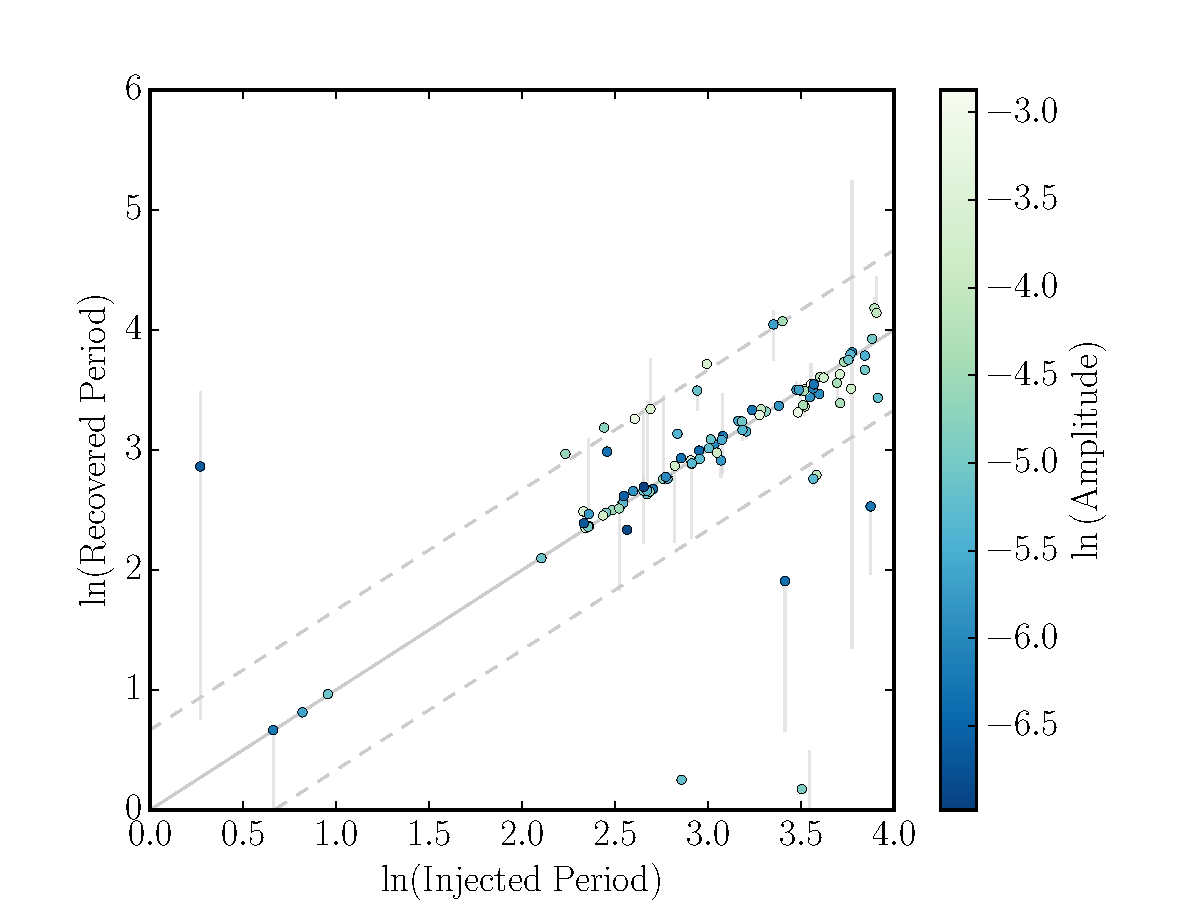
\includegraphics[width=6in, clip=true]{figures/compare_mcmc.pdf}
\caption{The `true' rotation periods used to generate \naigrain\
simulated light curves vs the rotation periods measured using the ACF
technique.}
\label{fig:compare_mcmc}
\end{center}
\end{figure*}

The marginal posterior distributions of the QP kernel hyperparameters for the
example simulated light curve with in figure \ref{fig:demo_lc}, are shown in
figure \ref{fig:gp_posteriors}.

\begin{figure*}
\begin{center}
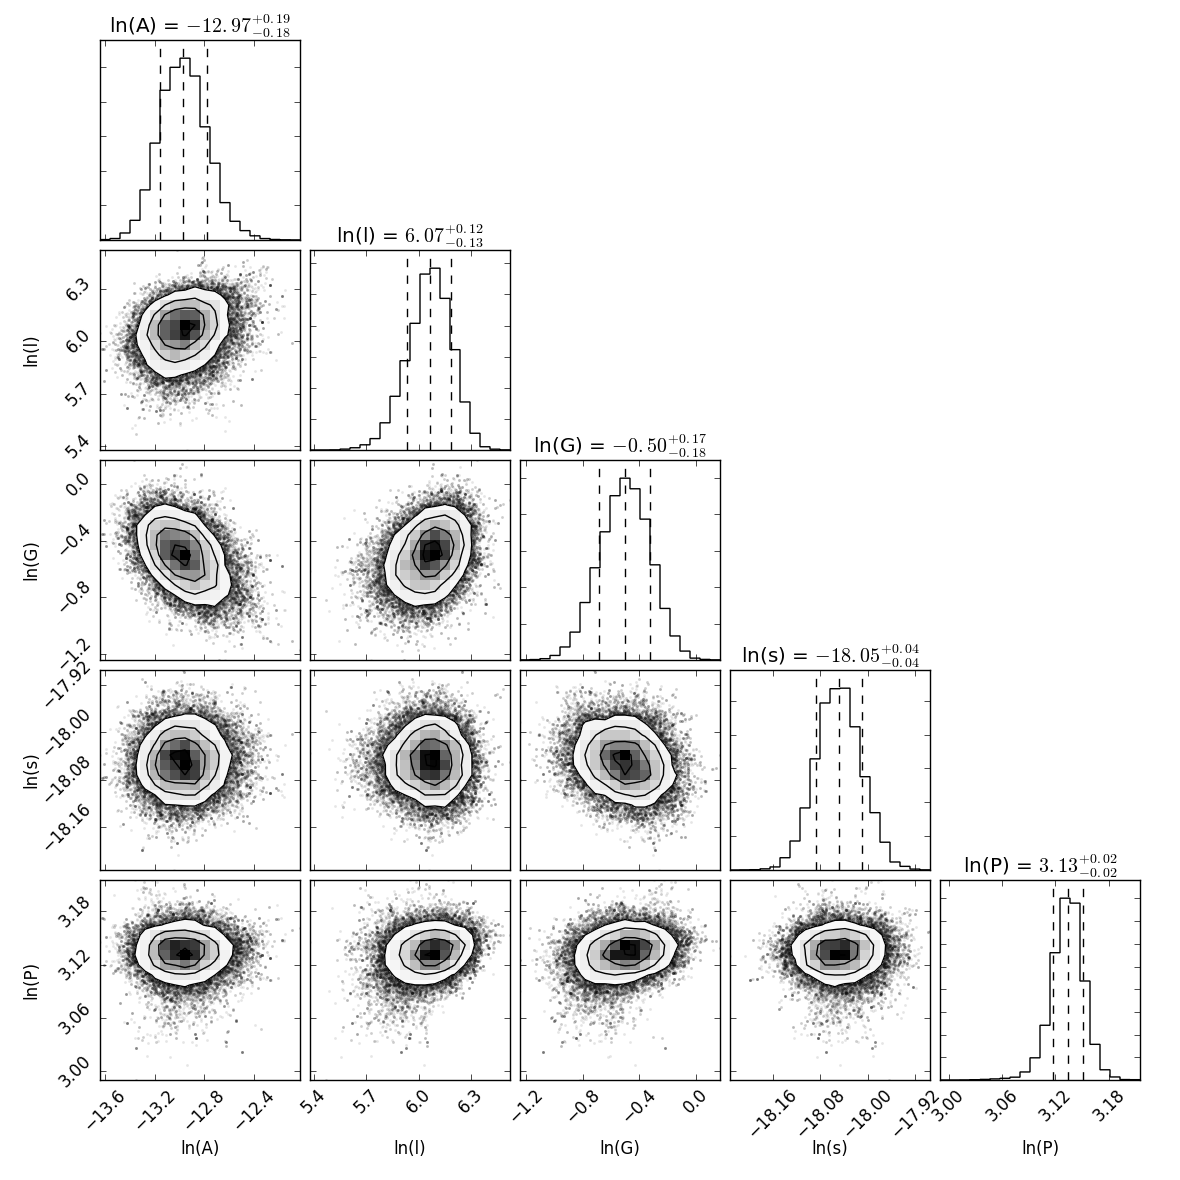
\includegraphics[width=6in, clip=true]{figures/0002_triangle.png}
\caption{(Place holder - to be updated.
Marginal posterior PDFs of the QP GP model parameters. $\sigma$ is an
additional white noise term added to the diagonal elements of the covariance
matrix. It is the fraction by which the observational uncertainties have been
underestimated. If the uncertainties reported on the data are too small, this
parameter will be non-zero.
The true rotation period of this star is ... ($\exp(...)$) days.}
\label{fig:gp_posteriors}
\end{center}
\end{figure*}

\section{Real \kepler\ data}
\label{sec:kepler}

We applied our method to \nmcquillan\ stars with rotation periods previously
measured by \citet{Mcquillan2014}.
A feature of \kepler\ light curves that works to our advantage is that they
are naturally broken up into smaller time units by quarterly (three month)
breaks.
As explained above, splitting the data set into quarters, rather than
modelling the entire time series contiguously speeds up the computation time
as inverting several small matrices is faster than inverting one large one.
The \kepler\ quarter divisions are natural places to split the time series
because the spacecraft rotates by ninety degrees every quarter (three months),
placing each star on a new CCD module.
Pixel response functions and background flux differs from pixel-to-pixel and
module-to-module, so noise properties of \kepler\ light curves change every
quarter.
Additionally, changes in the spacecraft's orientation and position during
quarterly re-pointings temporarily affect the temperature of the CCD,
producing systematic features in the light curves at the start of some
quarters.
We model each quarter separately but the parameters of the GP kernel function
are global, {\it i.e.} we do not use a separate period parameter for each
quarter---there is just one period parameter for an entire light curve.
It would be possible to model the time series with a mixture of some global
parameters and some quarter-specific parameters, for example one might expect
that the amplitude of covariance, $A$ or white noise level, $\sigma$ to vary
on a quarterly basis.
However, since there are seventeen quarters this would lead to thirty-seven
parameters, and in the interest of minimising computation time (adding
parameters leads to longer MCMC burn in and convergence time), we choose to
use global parameters only.

Our results show good agreement with the \citet{Mcquillan2014} measurements,
as shown in ... %\ref{fig:mcquillan}.

At this point it is important to highlight the following caveat.
Our method has been tuned to reproduce the rotation periods of the
\citet{Aigrain2015} simulated light curves.
These light curves were simulated using a very good but still imperfect model.
The input parameters and their distributions were chosen to be as realistic as
possible given current observations.
Unfortunately however, there are limited data on some of these parameters for
stars other than the Sun: for example the distrubution of spot lifetimes or
activity cycle length.
Ensuring that we can recover the rotation periods of these simulated light
curves does not necessarily ensure that we can recover the rotation periods of
real \kepler\ light curves with equal accuracy and precision.
Even using priors on the QP kernel parameters that have been derived from the
\citet{Aigrain2015} sample may be dangerous.
This caveat should be taken into consideration when this method is applied to
real data.

\section{Discussion}
\label{sec:discussion}

The main drawback of the GP method is computation time.
Because GPs are so expensive to compute, it is necessary to come up with
shortcuts in order to perform inference on \kepler\ light curves, each of
which compromises accuracy.
These shortcuts may only be necessary when working with a large number of
stars (of order hundreds or thousands).
If only interested in single or small numbers of targets it may be possible to
reduce the extremity of these shortcuts or to avoid them altogether.
The shortcuts that we employ here include:
\begin{itemize}
\item{Initialisation.
The choice of initial parameter values makes a difference to computation time:
the closer they are to the maximum likelihood parameters the shorter the MCMC
burn-in time.
Using the ACF period to initialise is not ideal as results will not be fully
independent of the ACF period unless MCMC chains are run for an infinitely
long time.}
\item{Subsampling.
Not only is some information always lost by subsampling, but the choice of
subsampling frequency will also effect the results.
We choose to retain an average of only 4 data points per day, based on the
range of rotation periods we are interested in.}
\item{Priors.
We choose to place a Gaussian prior in log-space over the rotation period
parameter where the standard deviation is twice the log of the ACF rotation
period.
Unfortunately however, if the true period is far different to the ACF period,
the MCMC chains will take a long time to reach the correct value.
In practice we found that the introduction of a Gaussian prior improved
results compared with a broad prior that was uniform in log-space.}
\end{itemize}

\subsection{Initialisation}
Using the ACF to initialise the MCMC chains is not ideal because, of course,
one becomes reliant on the assumption that the ACF period is close to the true
period.
Of course, if you had infinite CPU time, this would not be a problem as you
would eventually sample the entire posterior PDF of the period parameter,
however in practice this is likely to be an issue.
The only way to get around this problem is to run the MCMC chains for as long
as possible, or, alternatively to use a sampler that is designed to move
around the parameter space much more quickly than {\tt emcee}.
% We implemented a version of our code using nested sampling but the results
% were not as good as the {\tt emcee} method.
% We believe this to be due to the initialisation --- there is no initialisation
% in nested sampling, samples are drawn directly from the prior.
% In a problem with a multimodal posterior PDF such as inferring periods,
% initialising MCMC chains close to the maximum likelihood value may lead to a
% more rapid convergence.
We chose to use the ACF periods rather than the periodogram periods to
initialise the results since there were fewer large outliers.

\subsection{Kernel function choice and interpretation of hyper-parameters}
The QP kernel function represents a simplistic effective model of a stellar
light curve.
It adequately describes the data, captures that all-important periodic quality
and is relatively simple, with only a few hyper-parameters.
It also satisfies the requirement to produce positive semi-definite covariance
matrices.
Whilst the QP kernel function evidently captures the periodic qualities of
light curves adequately, it is still a somewhat arbitrary choice.
Another valid choice would be a squared cosine function multiplied by a
squared exponential,
\begin{equation}
k_{i,j} = A \exp \left(-\frac{(x_i - x_j)^2}{2l^2}\right)
\cos\left(\frac{2\pi}{P}\right)
\end{equation}
\label{eq:cos_kernel}
This function produces a positive semi-definite matrix and has the $P$
parameter of interest.
It may in fact be even {\it more} suited to modelling stellar
light curves as it describes a Gaussian in frequency space.
It is easy to imagine a differentially rotating star with a period that is a
Gaussian in frequency space: the mean frequency would be the frequency at the
most active latitude, at or near which spots spend the majority of their time
and the tails would be occupied by spots that drift near the equator or poles.
The main difference between this cosine and the QP function is that the cosine
function allows negative covariances and the QP function does not.
Is is realistic to allow negative covariances?
In practice, the ACFs of \Kepler\ light curves often go negative.
However, many stars have two active regions on opposite hemispheres that
produce two brightness dips per rotation.
If the covariance is forced to be negative for two data points that are
separated by half a rotation period, those light curves with two peaks per
rotation period may not be well modelled.
In other words, we do not want to force anti-correlation of points that are
$\frac{1}{2}$ a period apart.
It would be very worthwhile to test this assumption and this alternative
kernel function in future.
If CPU time were not limited there may be some benefit to performing formal
model comparison with different kernel functions.
However, the evidence integral is an ambitious calculation for models with
likelihood functions that take milliseconds to compute, let alone those
involving GPs with light curves containing thousands of data points which can
take minutes.

Clearly, stellar rotation periods are well represented by the $P$ parameter in
our QP kernel function, as evidenced by the its impressive ability to recover
the true rotation periods from the simulated light curves in this work.
However, it may not be the {\it best} function to use.
It is, after all, an approximation to the shape of the covariance matrix of a
real stellar light curve.
There may be an alternative function which is better suited to capturing
stellar variability and is able to recover periods even more precisely than
the QP kernel.
There may also be an alternative function which is more physically motivated,
that captures not just the rotation period but also (for example) the spot
lifetime or differential surface rotation.
This is beyond the scope of this work but we hope that these questions will be
answered in the near future.

Not all \kepler\ light curves show evidence of stellar rotation.
In some cases perhaps the star has few or no active regions, it is rotating
pole-on, or it rotates so slowly that the \kepler\ data detrending pipeline
removes any signal.
In other cases there may be another source of variability present in the light
curve, generating a false period detection.
These sources may be physical: \eg\ binary star interactions, intra-pixel
contamination from other astrophysical objects, pulsating variable stars,
asteroseismic oscillations in giants and even stellar activity cycles.
For some of these there is little we can do save attempt to eliminate these
astrophysical false positives via alternative methods, \eg\ apply colour cuts
to avoid giant contamination.
For some however, like the variable stars, they may have distinctive
hyperparameters that identify them, for example long coherence timescales.
Testing this is beyond the scope of this paper but may be an interesting
follow-up study.
As well as astrophysical contamination, there may also be instrumental sources
of contaminating variability: \eg\ temperature variations or pointing shifts
of the \kepler\ spacecraft.
These are unlikely to be periodic and, again, may produce unusual combinations
of hyperparameters.
This is something that we hope to test in future.
In addition to this, there are several other aspects of the GP method we hope
to test in future, listed as follows:.
\begin{itemize}
\item{To perform model selection with different kernel functions. Again, these
tests have not been performed due to the cost of calculating the fully
marginalised likelihood with GPs. This calculation may be prohibitively
expensive, however simpler model selection tests can be performed. For
example, the relative precision of rotation periods recovered using
alternative kernel functions could be tested.}
\item{To design and implement a physically motivated kernel function. We have
only explored the physical interpretation of one parameter in our kernel
function, $P$.
However, the other parameters may also be related to some physical processes.
For example, the overall timescale for covariance fall-off, $l$ may be
related to spot lifetimes.
A star with long spot lifetimes will show little variation in the overall
shape and amplitude of its light curve between rotations and $l$ will be
large.
In contrast, the light curve of a star with short spot lifetimes may display
non-repeating patterns and amplitudes that vary rapidly between rotations.
In this case $l$ will be small.
The $\Gamma$ parameter is related to the number of zero crossings within one
rotation period: when $\Gamma$ is small there are many zero crossings and
vice versa.
Since the number of zero crossings per rotation period is related to the
number of active regions on the surface of the star, this parameter may also
be of physical interest.
In addition, instead of interpreting the parameters of the QP kernel function
used here, it may be possible to design an entirely new kernel function, based
on the physical processes that drive the light curve variability.
This idea is being explored by another member of my research group.}
\item{To develop a detection criterion to assess whether a rotation period was
measured.
Another general problem in rotation period inference is deciding whether a
real rotation period was measured at all.
Detection thresholds are usually set using the amplitudes of peaks in LS
periodograms or ACFs in order to eliminate contaminants.
Using a GP model it may be possible to do this via model selection: \ie\ are
the data better described by a periodic model, or a non-periodic model?
There is more than one way to implement such a model comparison, one way could
be to use a sum of two kernel functions: one periodic and one non-periodic,
each with its own amplitude parameter.}
\item{To attempt to detect differential rotation.
We did not test our code on the light curves simulated with differential
rotation in \citet{Aigrain2015} since we were only interested in recovering
the most precise measurements of rotation period possible.
In future we intend to investigate the possibility of recovering
differential rotation by searching for close double peaks in the posterior
PDFs of stars' rotation periods.}
\item{To build in a noise model for \kepler\ data.
Another huge advantage of the GP method is, because it is a {\it generative}
model of the data, the rotation period signal can be modelled at the same time
as systematic noise features.
One can then marginalise over the parameters of the noise model.
This approach would be extremely advantageous for \kepler\ data since
long-term trends are often removed by the \kepler\ detrending pipeline.
Marginalising over the noise model at the same time as inferring the
parameters of interest will insure that the periodic signal is preserved.}
\end{itemize}

\section{Conclusions}

We used the \naigrain\ simulated \kepler-like light curves for solid-body
rotation from \citet{Aigrain2015} and attempted to recover the rotation
periods used to generate them.
Three methods were compared: a Lomb-Scargle periodogram method, an
autocorrelation function method and a new Gaussian process method.
The GP method produced the most precise and accurate rotation periods of the
three techniques.
This is because a GP is a semi-parametric model that is well suited to signals
that are non-sinusoidal and quasi-periodic.
Not only this, unlike the other two methods, the GP method provides posterior
PDF samples of rotation periods, allowing characterisation of uncertainties.
Note that the posterior PDFs are often non-Gaussian, being bi- or multimodal.
In these cases it is therefore misleading to report a 1$\sigma$ or 16th and
84th percentiles as uncertainties.
Rather, it is better to incorporate posterior PDF samples into analyses which
require uncertainty propagation.

Because rotation periods are inferred probabilistically with the GP method,
this allows them to be easily incorporated into follow-on studies; inferring
stellar ages or characterising star-planet interactions for example.
This the GP method also eliminates the need to define a heuristic detection
criterion such as are often used in the literature: a light curve that does
not contain a rotation signal will return the prior PDF.

The main drawback of the GP method is the computation time.

% acknowledgements
This research was funded by the Simons Foundation and the Leverhulme Trust.
Some of the data presented in this paper were obtained from the Mikulski
Archive for Space Telescopes (MAST).
STScI is operated by the Association of Universities for Research in
Astronomy, Inc., under NASA contract NAS5-26555.
Support for MAST for non-HST data is provided by the NASA Office of Space
Science via grant NNX09AF08G and by other grants and contracts.
This paper includes data collected by the Kepler mission. Funding for the
Kepler mission is provided by the NASA Science Mission directorate.

\bibliographystyle{plainnat}
\bibliography{GProtation}
\end{document}
